\documentclass{standalone}
\usepackage{tikz}
\usetikzlibrary{3d,arrows, calc, backgrounds, petri, positioning, shapes.geometric}

\tikzset{
	persp/.style={scale=3.0,x={(-0.8cm,-0.4cm)},y={(0.8cm,-0.4cm)}, z={(0cm,1cm)}},
	points/.style={fill=white,draw=black,thick}
	grid/.style={very thin,gray},
	axis/.style={->,blue,ultra thick},
	cube/.style={thick, fill=black!15,opacity=0.5},
	cube hidden/.style={dashed},
	block/.style={
		rectangle, rounded corners,
		draw=black!80,
		fill=black!10, fill opacity=0.5,
		text=black!90, text opacity=1.0,
    text height=1.5ex,
    text depth=.25ex,
    text width=6em,
    text centered
	}
}

\newcommand*{\rootPath}{../}

\begin{document}
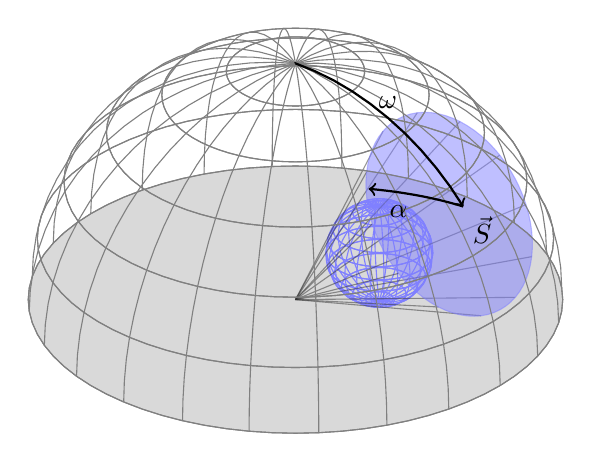
\begin{tikzpicture}[persp]

	\draw[gray,fill=black!15] (1,0,0)
	\foreach \rho in {5,10,...,355}
			{--({cos(\rho)},{sin(\rho)},0)}--cycle;

	\def\theta{-40}
	\def\phi{100}
	
	\def\scale{0.2}
	\def\distance{0.5}
	\pgfmathparse{asin(\scale/\distance)}\let\a\pgfmathresult

	\coordinate (X)				at (1,0,0);
	\coordinate (Y)				at (0,1,0);
	\coordinate (Z)				at (0,0,1);
	\coordinate (XS)			at ({	+cos(\phi)*cos(\theta)},	{ +sin(\phi)*cos(\theta)},	{ -sin(\theta)	}); 
	\coordinate (YS)			at ({	-sin(\phi)						},	{ +cos(\phi)						},	{ +0.0					}); 
	\coordinate (ZS)			at ({	+cos(\phi)*sin(\theta)},	{ +sin(\phi)*sin(\theta)},	{ +cos(\theta)	});
	\coordinate (obj)			at ($\distance*(XS)$);
	
	\foreach \t in {5,20,...,170}
	{
		\draw[blue!50] ($(obj)+\scale*({cos(\t)},{sin(\t)},0)$)
		\foreach \rho in {5,10,...,360}
			{--($(obj)+\scale*({cos(\t)*cos(\rho)},{sin(\t)*cos(\rho)},{sin(\rho)})$)};
	}
	\foreach \t in {0,15,...,345}
	{
		\draw[blue!50] ($(obj)+\scale*({cos(\t)},0,{sin(\t)})$)
		\foreach \rho in {5,10,...,355}
			{--($(obj)+\scale*({cos(\t)*cos(\rho)},{cos(\t)*sin(\rho)},{sin(\t)})$)}--cycle;
	}	
	
	\foreach \t in {10,40,...,340}
	{
		\draw[black!80, opacity=0.5] (0,0,0)--($cos(\a)*(XS)+cos(\a)*tan(\a)*cos(\t)*(YS)+cos(\a)*tan(\a)*sin(\t)*(ZS)$);
	}
	\fill[blue!50, draw, opacity=0.5] ($cos(\a)*(XS)+cos(\a)*tan(\a)*(YS)$)
	\foreach \t in {5,10,...,355}
	{ --($cos(\a)*(XS)+cos(\a)*tan(\a)*cos(\t)*(YS)+cos(\a)*tan(\a)*sin(\t)*(ZS)$) }--cycle;


	\foreach \t in {5,20,...,170}
	{
		\draw[black!50] ({cos(\t)},{sin(\t)},0)
		\foreach \rho in {5,10,...,180}
			{--({cos(\t)*cos(\rho)},{sin(\t)*cos(\rho)},{sin(\rho)})};
	}
	\foreach \t in {0,15,...,165}
	{
		\draw[black!50] ({cos(\t)},0,{sin(\t)})
		\foreach \rho in {5,10,...,355}
			{--({cos(\t)*cos(\rho)},{cos(\t)*sin(\rho)},{sin(\t)})}--cycle;
	}



	%% \draw[->,thick,black]	(0,0,0)--(XS) node[black,above right]	{$\vec{S}$};
	\draw	(XS) node[black,below right] {$\vec{S}$};
	
	\draw[->,thick,black]				($(XS)$)
	\foreach \t in {1,2,...,\a}
	{ --($cos(\t)*(XS)+sin(\t)*sin(-50)*(YS)+sin(\t)*cos(-50)*(ZS)$) };
	\draw ($cos(\a/2)*(XS)+sin(\a/2)*sin(-50)*(YS)+sin(\a/2)*cos(-50)*(ZS)$) node[black,below left] {$\alpha$};
	
	\draw[->,thick,black] ($(Z)$)
	\foreach \t in {-90,-85,...,\theta}
	{ --({cos(\phi)*cos(\t)},{sin(\phi)*cos(\t)},{-sin(\t)}) };
	\draw ({cos(\phi)*cos((\theta-90)/2)},{sin(\phi)*cos((\theta-90)/2)},{-sin((\theta-90)/2)}) node[black,above] {$\omega$};




	
	
\end{tikzpicture}
\end{document}